%!TEX root = ../../../thesis.tex
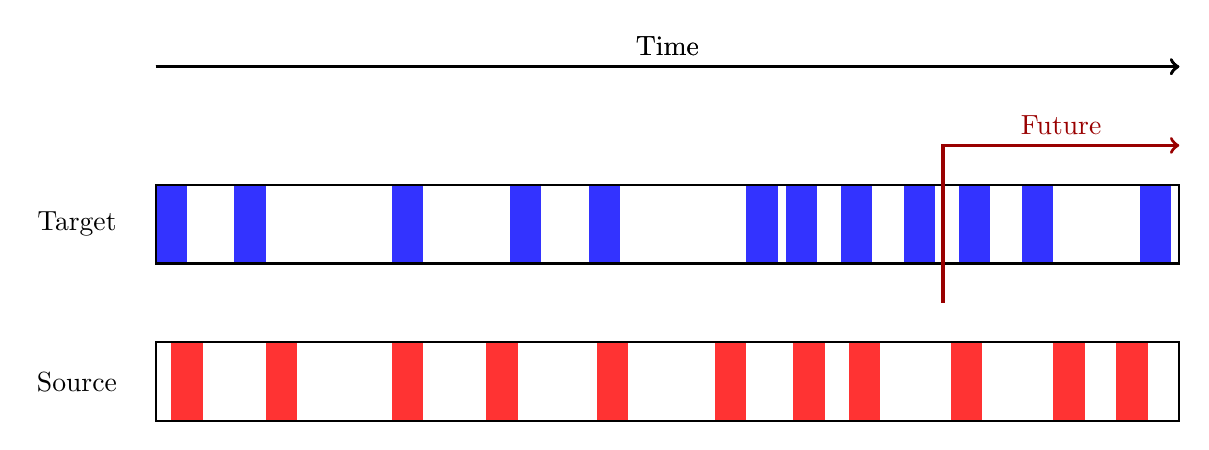
\begin{tikzpicture}
	
	\node at (-1, 0.5) {Target};
	\node at (-1, -1.5) {Source};
	
	
	%% BLUE EVENTS
	% Main
	\draw [thick] (0,0) rectangle (13,1) ;
	
	% Events
	% Past Events
	\foreach \x in {0, 1, 3, 4.5, 5.5, 7.5, 8, 8.7, 9.5}
	{
		\fill[blue!80!white] (\x,0) rectangle ++(0.4,1);
	}
	% Future Events
	\foreach \x in {10.2, 11, 12.5}
	{
		\fill[blue!80!white] (\x,0) rectangle ++(0.4,1);
	}
	
	% Redraw Main Rectangle
	\draw [thick] (0,0) rectangle (13,1) ;
	
	
	%%ORANGE EVENTS
	
	% Main
	\draw [thick] (0,0) rectangle (13,1) ;
	
	% Events
	% Past Events
	\foreach \x in {0.2, 1.4, 3, 4.2, 5.6, 7.1, 8.1, 8.8}
	{
		\fill[red!80!white] (\x,-2) rectangle ++(0.4,1);
	}
	% Future Events
	\foreach \x in {10.1, 11.4, 12.2}
	{
		\fill[red!80!white] (\x,-2) rectangle ++(0.4,1);
	}
	
	% Redraw Main Rectangle
	\draw [thick] (0,-2) rectangle (13,-1) ;
	

	
	% Time Arrow
	\draw [very thick, ->] (0,2.5) -- (13,2.5) node[midway, above] {Time} ;
	
		% Future
	\draw [red!60!black, very thick, shorten >= -0.6pt]        (10,-0.5) -- (10,1.5);
	\draw [red!60!black, very thick, ->] (10,   1.5)  -- (13, 1.5)   node[midway, above] {Future} ;
	% Now
%\draw [red!60!black, very thick, shorten >= -0.6pt]        (10,-0.2 ) -- (10,1.2) node[above] {Now};
	
	% Time Arrow
	\draw [very thick, ->] (0,2.5) -- (13,2.5) node[midway, above] {Time} ;
	
%	% Past brace
%	\usetikzlibrary{decorations.pathreplacing}
%	\draw [very thick, -, draw=black, decorate, decoration={brace,amplitude=10pt,mirror,raise=4pt} ] (9.8,1) -- (0.2,1)
%	node[midway, above, yshift = 14pt] {Past} ;
	
\end{tikzpicture}